\section{Validation and Calibration}
\label{sec:validation}

\paragraph{Pathfinding benchmarks.} A* was benchmarked on the official challenge maps by
computing, from a random start, the path to every valid tile, averaged over 300 iterations per
map (MacBook Pro M1 Max):

\begin{table}[htbp]
\centering
\footnotesize
\begin{tabular}{lrr}
\toprule
Map & Time (ms) & Valid tiles \\
\midrule
\texttt{empty\_30} & 21.45 & 900 \\
\texttt{circuit\_directional} & 16.20 & 485 \\
\texttt{hallways\_interconnected} & 8.56 & 465 \\
\texttt{caothic\_maze} & 7.16 & 432 \\
\texttt{wide\_path} & 12.14 & 526 \\
\texttt{two\_obstacles} & 11.36 & 524 \\
\texttt{crates\_one\_way} & 0.31 & 47 \\
\bottomrule
\end{tabular}
\caption{A* pathfinding: total time to reach every valid tile from a random start. With move
durations of at least 50\,ms, planning always fits well within a single movement tick.}
\label{tab:astar}
\end{table}

\paragraph{Data-driven fuzzy/MCTS calibration.} Rather than hand-guessing constants, the live
agent was instrumented: a one-time dump of the server-provided game configuration, a periodic
\texttt{[FUZZY-CALIBRATE]} log recording observed min/max cost, reward, and score per desire
category against the active fuzzy scale, and a per-search \texttt{[MCTS-CALIBRATE]} log
recording root branching factor, total visits, and the top visited children. This surfaced and
fixed several concrete issues: cost breakpoints moved from the Euclidean diagonal (real A* costs
reached 58 on a $30{\times}30$ map, past $\sqrt{w^2+h^2}\approx 42$) to $w+h$; reward
breakpoints were made robust to zero-variance reward distributions; delivery and exploration
desires that silently reported a zero reward signal were repaired; and dead risk rules were
removed. On the MCTS side, calibration revealed that the effective bottleneck was not the UCB1
constant but the root branching factor (57--95 children, dominated by per-spawner exploration
desires): with 100 iterations, UCB1's forced first visit to every child consumed most of the
budget, and visit concentration improved sharply whenever branching dropped. This motivates the
exploration-desire aggregation discussed in Section~\ref{sec:future}.

\paragraph{Scenario testing and observability.} The BDI agent was validated on the Challenge~1
scenario maps (including the crate-blocked \texttt{crates\_one\_way} map exercising the PDDL
pathfinder), and the LLM agent on Challenge~2 atomic-request scenarios through the chat
interface. A live terminal UI (Figure~\ref{fig:bdi-log}) renders the full deliberation state ---
belief grid, current desire set with evaluations, the change-detection strategies that triggered
the last cycle, and the committed intention with its fuzzy score --- which proved essential both
for debugging emergent behaviour and for the calibration campaign above.

\begin{figure}[htbp]
    \centering
    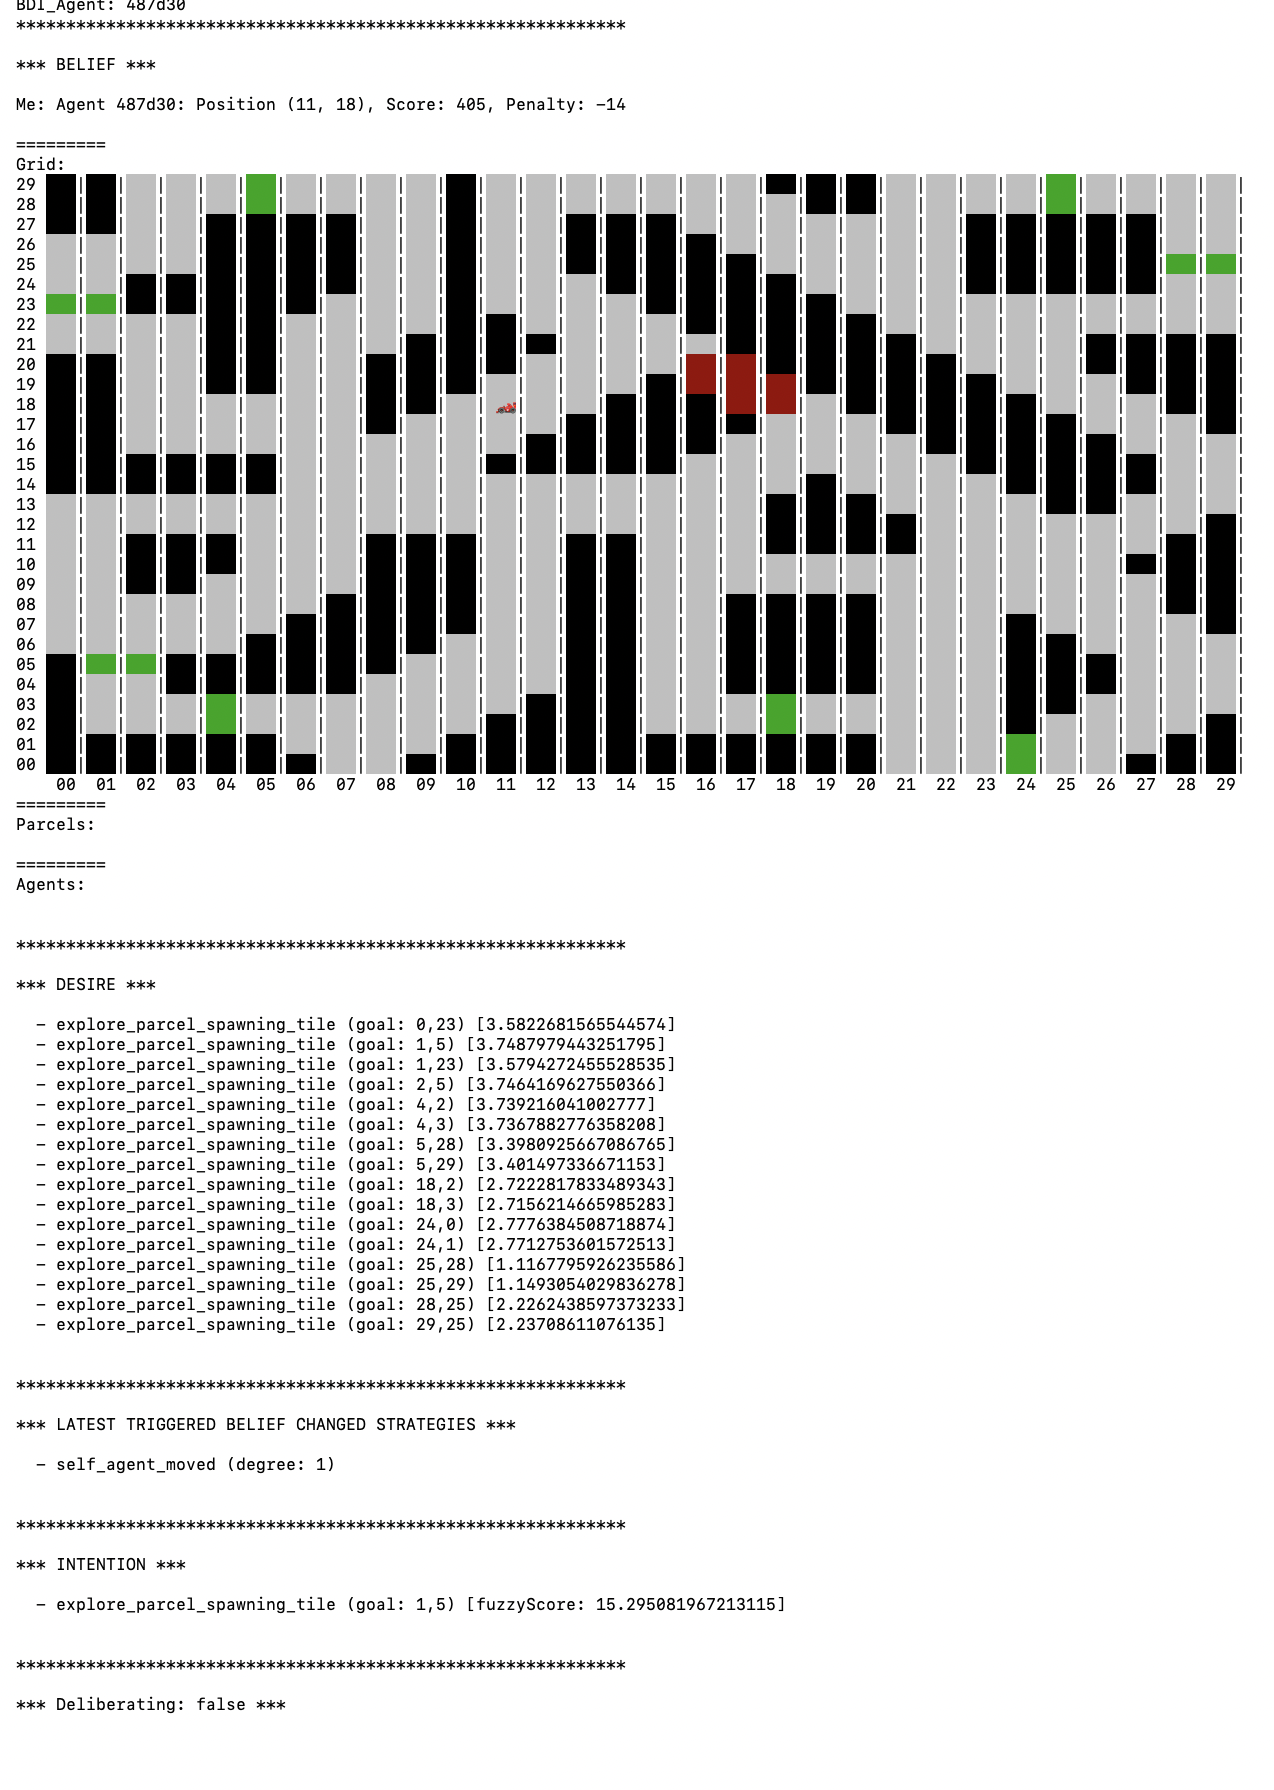
\includegraphics[height=12.6cm,keepaspectratio]{figures/bdi_log.png}
    \caption{Live terminal UI of the BDI agent on a $30{\times}30$ map: belief grid (agent,
    walls, spawner and delivery tiles), the generated exploration desires with their staleness
    evaluations, the change-detection strategies fired on the last belief update, and the
    committed intention annotated with its fuzzy desirability score.}
    \label{fig:bdi-log}
\end{figure}
